\part{Towards Highly Miniaturized LED Power Systems }
\label{ch:twrd_HMLED}

\chapter{LEDification: The second lighting revolution}


The light bulb was one of the most relevant inventions form our past history.  Electrical lighting was definitely a revolution in the early 19$^{th}$ century society; for the first time in the history, human kinds had a clear, reliable and safe source of artificial light that was easy to distribute and control. The apparition  of the electrical light bulb was also, with no doubt, the trigger for the commercialization of electric power and the deployment of the first power distribution networks.  The impact in the humans was to such degree that it settled two of capital sectors from the present industry network, the lighting and the electric power distribution, with  world recognized companies such as Philips, General Electric or Osram.  Actually, both sectors have been so close related that even often we use the word \emph{light} when we actually are refereing electricity. In resume, one single invention changed our society for ever, bringing light and electricity to our homes.

\begin{figure}[!h]
\centering
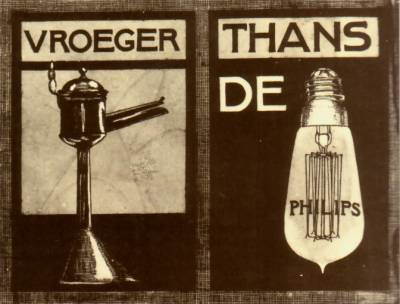
\includegraphics{./0_intro/img/1900-philips3.jpg}
\label{fig:incandescent_light_blub}
\caption{Early incandescent light bulb}
\end{figure}


From the initial invention of the first incandescent light bulb,  bulbs have just been illuminating our daily lives with any special \emph{enlightening} relevance of innovation and research from the rest of the humans. Despite our impression,  important research have been done to improve the worst characterises of an incandescent light bulb, the efficacy. Incandescent light bulbs are extremely bad in generating light with a luminous efficacy ranging between $12.6 lm/W$ for the tungsten incandescent to $24 lm/W$ of the quartz halogen. Bringing the numbers to a more comprehensive way, we can say that in general incandescent lights convert at least 95\% of the supplied power in heat and just, at most 5\% in light. If we combine that numbers with the fact lighting consumes one third of the total produced electrical power, we can account that 30\% of the total produced power is transformed in to heat and only a 3\% is transformed in real light\note{These figures projected assuming all lighting is produced by incandescent light bulbs, \emph{thanks god} that is nor longer true thanks to the energy efficient light  bulbs}. Thus form these figures we can understand  the motivation and necessity of improving the efficacy of the light bulbs.

Gas-discharge lamps where the first alternative of the incandescent lamps benefiting with a better efficacy, being the fluorescent tub the most popular among the family. The low pressure mercury-vapor gas-discharge  lamp, florescent tube, could be considered an innovation in the lighting. Initial the tubs where mainly used for big spaces warehouses, factories and offices, and later one, in the late 80's, started populating domestic houses with the appearance of the \emph{compact fluorescent lamps}\note{Screw-in version of a fluorescent tube. Now a days you can find a CFL replacement for almost the majority of sockets in the market.} (CFLs), being now a days the market standard for energy efficient light bulbs. Florescent lamps are indeed a big improvement in efficacy with respect to the incandescent lamps. The luminous efficacy ranges between 52-100 $lm/W$, depending on the light color temperature, converting about 22\% of the input power to visible light, more details of other gas-discharge bulbs is presented in Table\ref{tab:light_sources}. Although the better efficiency of the gas-discharge lamps, they did not fully replace the inefficient incandescent ones due some disadvantages; the most two main aspects poor light quality, light color is not nice and it derates over time and the slow turning time, lights take few minutes to produce full light.

Being the florescent lamps one of the biggest contributions during the past century, beginning  to be commercialized around 1930. Later becoming a disruptive change in the lighting market with the introduction the low consumption lamps where Philips was one of the first player launching to the market the first screw-in fluorescent lamp. Although the prices of these lamps has been dropping to become commercially attractive for the costumers, their poorer color rendering factor and the longer setting time compared to the incandescent lamps prevented this lamps to be one-to-one replacement. Therefore the lighting industry has been keep without not too much attention till the introduction the LED based lamps. 



\vspace{5mm} %5mm vertical space

\begin{figure}[!h]
\centering
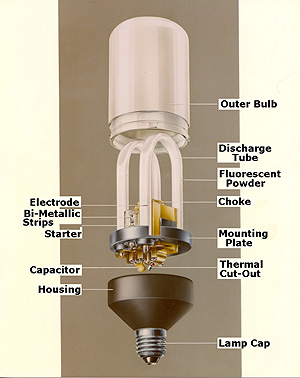
\includegraphics{./0_intro/img/phil1b.jpg}
\label{fig:philips_sl}
\caption{Components of the Philips SL compact fluorescent lamp. }
\end{figure}

The discovery of the high-efficiency blue LED ~\cite{94Nakamura} by Shuji Nakamura in 1994 enabled the quick development of the fist efficient withe LED. These early high power LEDs demonstrated that Solid State Lighting (SSL) devices  where a suitable technology for illumination. The relevance of Nakamura's work has been recognized last year being him awarded with the 2014 Nobel prize in physics. Looking farther we can also confirm the relevance of his invention since the apparition of the LED lamps, lighting is impacting again in our everyday life by changing our traditional concept of luminaries and lighting possibilities.

\begin{figure}[!h]
\centering
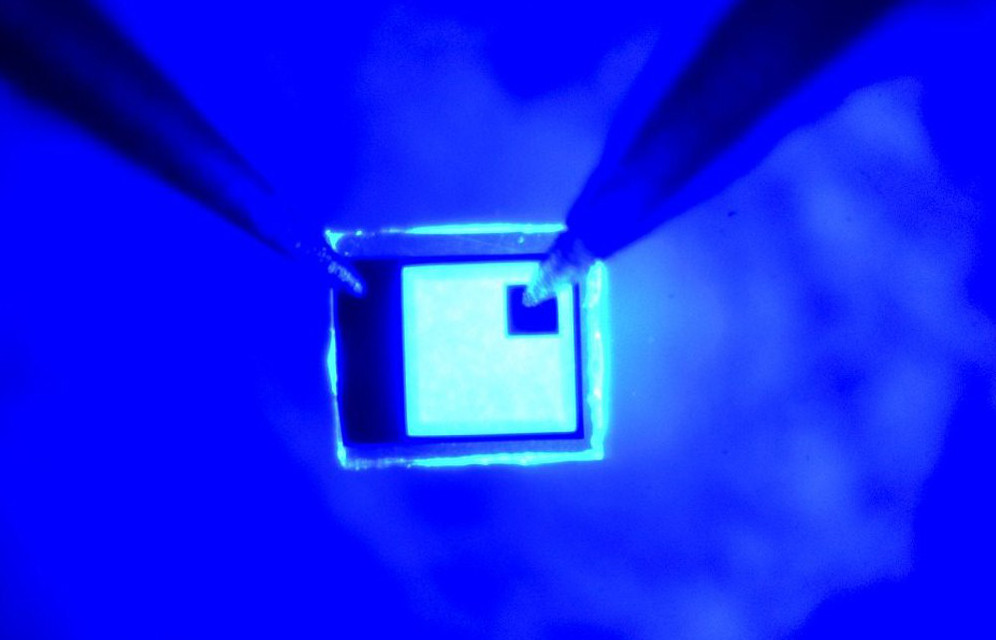
\includegraphics{./0_intro/img/10-7-14-nobel-prize-blue-led.jpg}
\label{fig:blue_LED}
\caption{Picture of a blue LED researched by Shuij Nakamura.}
\caption*{Source: \url{http://www.newsweek.com/how-blue-led-changed-world-and-won-nobel-prize-275977} }
\end{figure}

LED based lamps triggered  a frenetic rush in the lighting industry to bring that technology to the end consumers. Actually the large number of advantages of LED based lighting, or also known as Solid State Lighting (SSL), are so relevant that in the close future will replace any of the present lighting technology, that movement has been already named as the \emph{LEDification}. The principal advantages of SSL are:
\begin{description}
  \item [Efficiency] The light generation inside an LED is produced by the direct mechanism of hold-electron recombination, the supplied energy is a better use of the energy compared to the incandescent lamps. The power consumption can be up to an order of magnitude lower of an incandescent light.

  \item [Size] LEDs are tiny and flat devices, which can be considered as 2-D elements and do not need any vacuum chamber to work. They are much more flexible devices to assembly, and can easily replace the old glass made bulb design.

  \item [Color] LED light has a very narrow light spectrum, that can be used to produce directly colored light. Colored lights are becoming more popular in domestic homes becoming a piece of decoration or mood tweaking device.

  \item [Dynamics] Compared to any of the traditional sources of light LEDs have no dynamics, actually they have but it's very fast and not appreciable to the human eye. Therefore they do not have any setting time when turned on, which is not the case of CFL. The fast dynamics allows to modulate the light and transmit data without disturbing the human beings.

  \item [Lifetime] Solid State devices do not wear off, there fore they can be considered to have an infinite lifetime. In practice LEDs make use of organic phosphores, thus the light quality derates with the use, but the life expectancy of the LED is rated from 20.000 - 100.000 hours, multiplying 20 to 100 times longer that the classical light bulbs.
\end{description}

\vspace{5mm} %5mm vertical space

Bring the LED based lamps to the market is still a big challenge. Despite of the large number of advantages, the end consumers are still very reluctant to change generally due to the elevated costs of the new lamps, currently ranging between \$20 - \$40 for a 100W substitute compared to less than \$3 of an incandescent light. Also another issue that prevents consumers to change to the new technology is a poor light color consistency, light flickering and light dimming incompatibilities, that become really evident in low budget products.

\begin{figure}[!h]
\centering
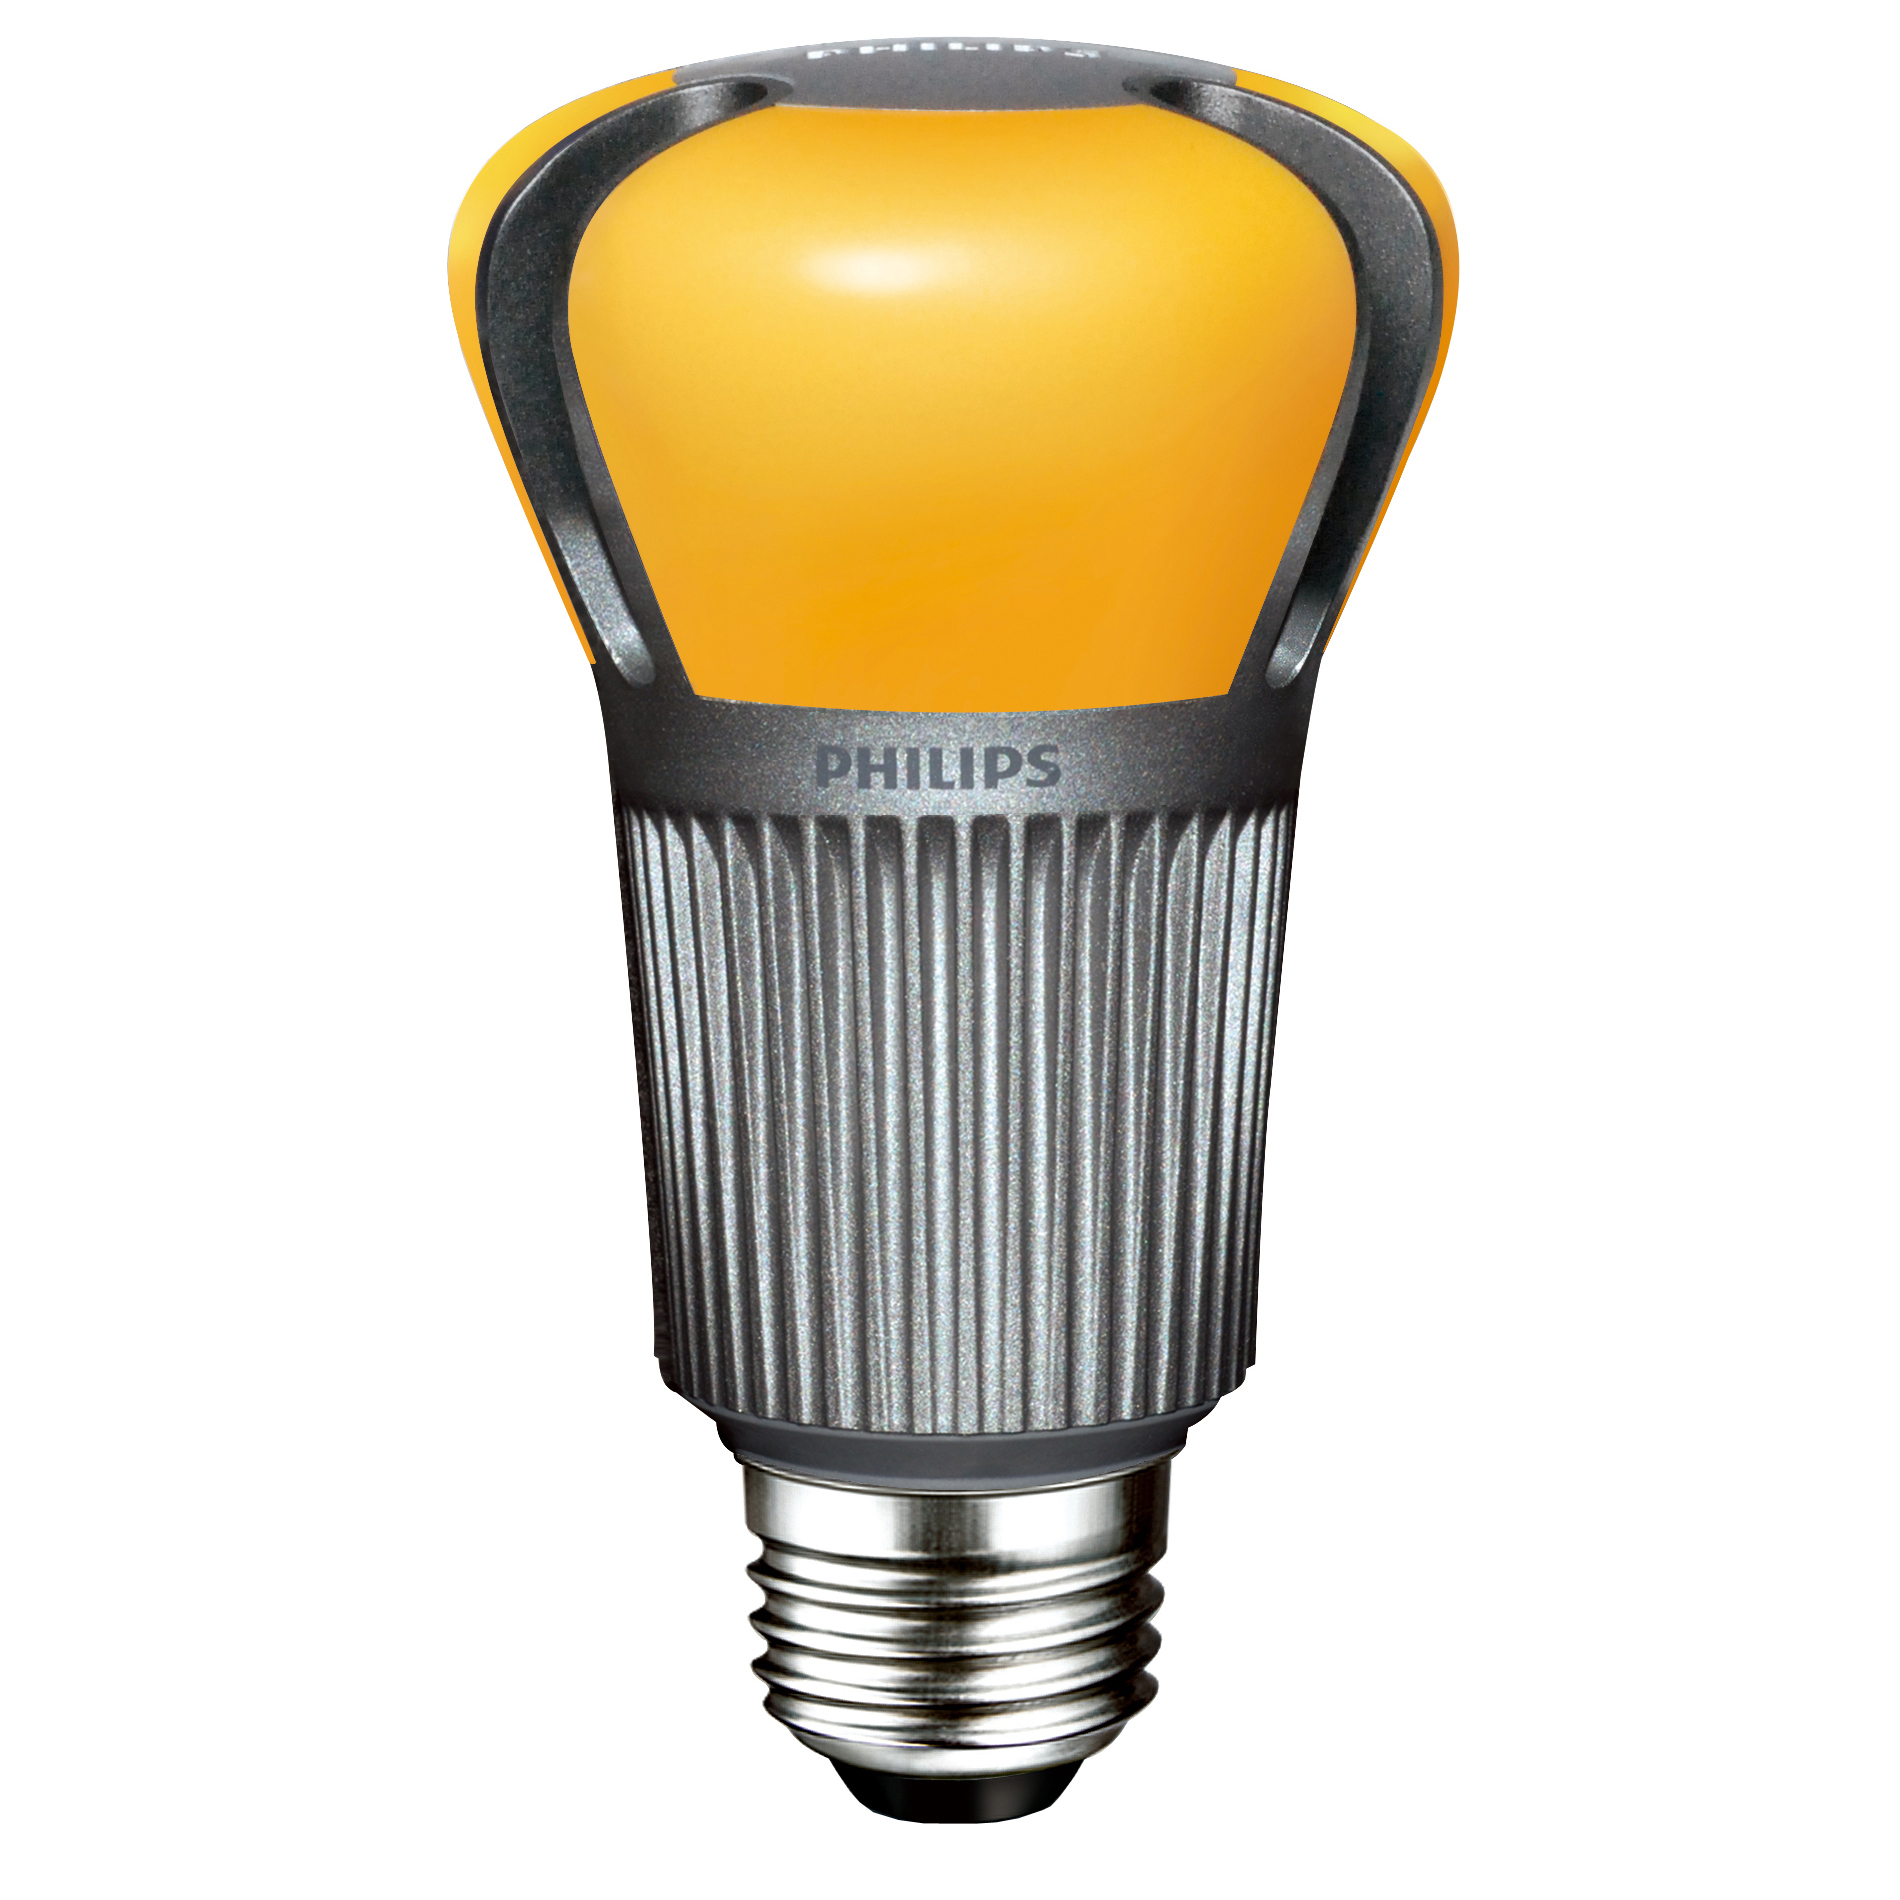
\includegraphics[width=4cm]{./0_intro/img/enduraled-12w.jpg}
\label{fig:l_prize}
\caption{900 lumens LED light bulb.}
\end{figure}

Two factors can be identified to make more favorable the adoption of the SSL as the preferred lighting solution by the consumers. In the one hand, reducing the end product price; and in the other hand, bringing more value to the traditional light sources. Actually LED light bulbs already bring more value compared to the old light bulbs being much more efficient, almost one order of magnitude lower in power consumption, and a longer lifetime, easily twenty times more operating hours. However these factors are not yet a valuable argument for the consumers. With the current trend of the \emph{internet-of-things} remote control, color tuning, light level dimming and integration to with future smart houses are probably some value propositions that people will need and SSL can easily provide. In a second level, I assume that the luminaries designs will change with a more favorable designs that take advantage of the low profiles of the LEDs.

 \begin{figure}[!h]
\centering
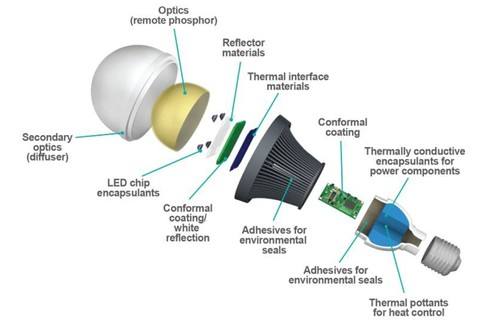
\includegraphics[width=8cm]{./0_intro/img/exploded_bulb_2.jpg}
\caption{Exploded vision of an LED light bulb.}
\label{fig:exploded_bulb}
\end{figure}

It is essential to describe the different elements in a LED light bulb in order to understand the challenges in its development and  design. A LED light bulb is composed by the six main elements described below and shown in  the Fig. ~\ref{fig:exploded_bulb}.

\begin{description}
  \item[LED] A two-lead semiconductor device that produced light when a current flows through it. The name comes from its acronym \emph{Light-Emitting Diode}. The light is produced by electroluminescence when an electron recombines with an electron-hole releasing energy in form of photons. The color of the light is determined by the energy band gap of the semiconductor.

   LED cost is very cheap and there is a broad assortment in colors, power and applications. The selection of the LED will determine: light color, voltage and current of the load, efficiency and necessary optics.

  \item[Optics] The optical device that helps to collimate, mix and distribute the light in the space in a desired way, normally uniformly for a determined projection area.

  \item[Driver] Electronic circuit placed between the input source and the load, the LEDs, that transforms the input electrical power to the requirements of the load. Since almost all the power distribution systems and storage devices are voltage sources and LEDs are current supplied loads, an LED driver is considered as current-to-voltage (V-I) power supply.

      The driver controls the current thought the load, hence the light output. Therefore it can be considered as the active part of the system where the control of the lamp relies. It is the most expensive and takes the largest volume of the lamp, and also one of the most or even the most important element in the entire system.

  \item[Heat sink] Mechanical element that acts as a passive heat exchanger and cools hot elements within the lamps system by dissipating the heat into the surrounding medium. The energy that is not converted to light becomes heat and must be extracted from the lamp, the main heat contributors elements are the LEDs and some components of the driver.

      The costs of the heat sink is also a relevant part in the total cost of the lamp.

  \item[Body assembly] Mechanical element that hold all the different subsystems in one single device. In many cases the heat sink does this functionality.

  \item[Connector] Mechanical element that provides connection with the energy source. The most popular one is the Edison connector present in all screw-in lamps. There are many other popular ones such as GU10, MR16, MR11 coming from the halogen multifaceted reflector bulbs or the 2-pin connector of the fluorescent tubes.

      In many cases, the standardized connectors suppose a restriction for the mechanical design of the lamp. Their old-fashioned design is not optimal for the new lamps.


\end{description}

\vspace{5mm} %5mm vertical space

The chart shown in Fig.\ref{fig:cost_breakdown} makes evident that the driver is the most expensive part of the system. As it was previously mentioned, the driver is the key component in the functionality of the LED lamp, since it controls the light output and at the same time determines the efficiency of the system. Therefore, the LED driver has become on of the hot topics of research within the power electronics field. Besides the necessity of fulfilling the operational requirements, such as high efficacy an proper power quality, two main issues have trigger research around the driver circuit: The costs and the volume.
\begin{figure}[!h]
\centering
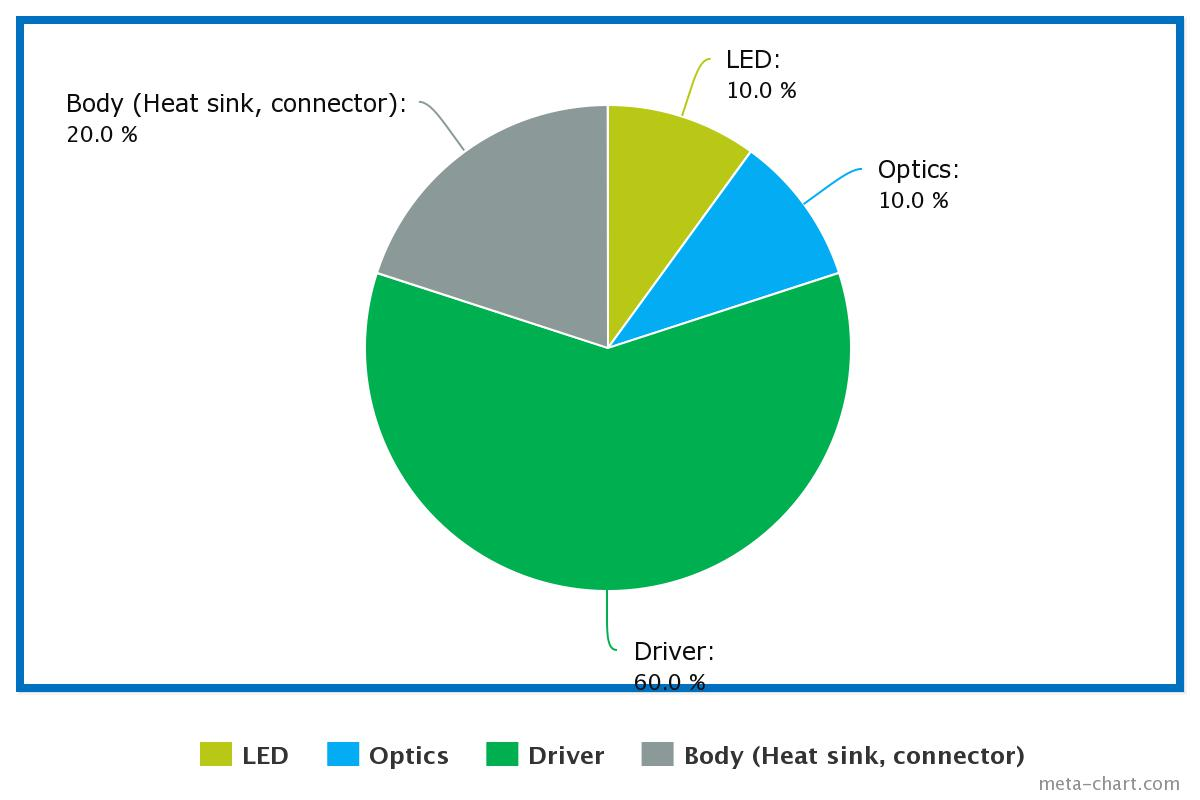
\includegraphics[width=8cm]{./0_intro/img/piechar_costs.jpeg}
\caption{LED lamp cost breakdown by subsystems.}
\label{fig:cost_breakdown}
\end{figure}

\vspace{5mm} %5mm vertical space

The cost of the driver is one of the biggest problems that SSL industry has been dealing after the power LEDs become a commodity components. Actually, this piece of electronics was not present in the incandescent light bulbs, thus its elevated cost arose as an inconvenient and difficult to justify in the new light bulbs. Philips Research has devoted a large effort in that field, being indeed the main focus of research regarding the LED drivers.


Reducing the costs of the lamps has been the strategy taken for the first wave in the \emph{LEDification} process where retrofitting\footnote{Adding the new LED technology to the older light bulb systems. In that way the end user can directly replace an incandescent lamp or a florescent tub by an LED one without needing to make any change in the current installation.} the old lamps is chosen as the way to target the end costumer. In on the one hand, fruitful results came form that research with new innovative solutions at very low costs that could be packed in almost all the light bulb shapes currently commercially available. But in the other hand, these new drivers had the incontinent of using very old components that at the same time restricted reduction of the circuit volume and made more complex the addition of extra control functionalities while keeping the initial low costs.

\begin{figure}[!h]
\centering
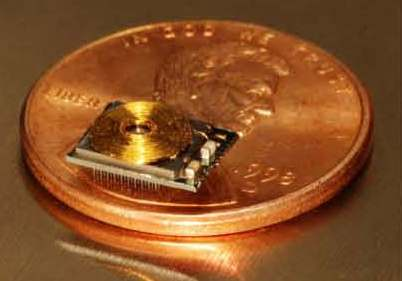
\includegraphics[width=8cm]{./0_intro/img/FSolzbacher01.jpg}
\caption{Power System in a Package die. The circuit implements a buck converter.}
\label{fig:psoc_example}
\end{figure}

\vspace{5mm} %5mm vertical space

The second line of research has focus on reducing the volume of the driver circuit. That research topic arose when comparing the the volume of the LEDs and the driver, it is evidenced a mismatch between the two volume of the components, becoming in many cases the driver circuit the dominant element of the entire lamp. Such mechanical constrain supposes an obstacle to take the full advantage of the low form-facto of the LED in the future luminaries, where LED will not be assembled using the old fashioned cases. Therefore, that research has a much longer term vision for targeting the second of third generation of lights in the \emph{LEDification} process.

The drive to reduce the volume of the drivers led to focus the research from the perspective of the integrated power supplies, where the power converter can be partially or fully integrated in a single package. There are two approaches of integrated power converters: \emph{Power System on Chip} (PSoC) or  \emph{Power System in Package} (PSiP). The first integrate all required power components, active and passive, in a single die. The second assemble all the components within the same package, keeping the appearance of an unique \emph{Integrated Circuit} (IC), see Fig.\ref{fig:psoc_example}. The advantages of having an integrated power management unit align with the necessities of the LED drivers, therefore trend of the drivers will be going towards having \emph{Power LED Drivers in Package} (PLDiP).

Besides the size reduction that an integrated driver would suppose, an integrated approach would also bring other benefits in terms of control and connectivity. Since such a solution would require a the design of a dedicated \emph{application-specific integrated circuit} (ASIC), the power management unit and driver control unit can be integrated together, providing the necessary intelligence for light control and the connectivity optimized for the requirements of the coming connected lighting industry. The \emph{Philips} \emph{HUE} lamp is a clear example of the requirements of the so called \emph{smart drivers}. That lamp provides a full light color gamut color control through a mobile and web application or through a remote control. The internal driver has four light channels red, green, orange and additional amber and at the same time provides wireless connectivity through ZigBee, being the electronic board populated with discrete power drivers and few micro-controller units. A solution that integrates all the functions in a single IC, or few ICs (one per channel), will definitely reduce packaging and assembling costs and still providing the same functionalities. And at the same time, the expected market size for LED lighting to justify a dedicated ASIC design for the light bulbs and indeed has been the motivation of this thesis. Therefore goal of this work was to explore and identify new architectures that are suitable for integration and at the same time can perform as an efficient LED driver.


\section{Why a LED needs a driver?}

As shown in Fig. \ref{fig:led_I-V} a LED has a very abrupt V-I curve. For voltages below the \emph{forward voltage}, $V_{f}$, there is no current flow and the LED behaves as an open circuit. For voltages above $V_{f}$ the curve becomes very steep and the current increases dramatically with respect to the voltages, thus the LED behaves as short circuit. The driver bias the LED to a specific point, $P$ in Fig. \ref{fig:led_I-V}, providing the desired output light. The colour and flux (light intensity) will vary depending of the bias point.  Since the majority of  available  energy sources are  voltage sources, and LED requires a circuit that limits the current that flows through it, that circuit is the LED driver.

\begin{figure}[!h]
\centering
\begin{tikzpicture}[domain=0:5]
    \draw [->] (0,0) -- (4.5,0) node[anchor=west]{$V$};
    \draw [->] (0,0) -- (0,4.5) node[anchor=east]{$I$};

    %Mark Vth
    \draw (2,2pt) -- (2,-5pt) node[anchor=north] {$V_{f}$};

    %Draw ideal plot
    \draw[thick] (0,0) -- (2,0) -- (4,4);

    %Draw bias points
    \draw[dashed] (3,2) -- (3,-0);
    \draw (3,2pt) -- (3,-5pt) node[anchor=north]  {$V_{bias}$};

    \draw[dashed] (3,2) -- (-0,2);
    \draw (2pt,2) -- (-5pt,2) node[anchor=east]  {$I_{bias}$};
    \filldraw (3,2) circle(2pt) node[anchor=west] {$P$};



\end{tikzpicture}
\caption {}
\label{fig:led_I-V}
\end{figure}

At the first glance, keeping a constant bias current, $I_bias$, through the LED does not seems to be challenging. However LED V-I characteristic is not static, in practice LEDs has different source of deviations and drivers have to deal with them in order to keep delivering the desired light output. First, $V_f$ has a negative dependence with the temperature, drooping its values as the PN junction temperature increases. Second, the LED has an aging factor derating its light output over time, which has to be adjusted by changing the bias point. And last but not least, during production LEDs will vary in colour, flux and forward voltage; even for products from the same batch. The manufacturer reduced the dispersion between devices by binning \footnote{Quality control performed at LED production line, where each LED is individual tested and sorted in groups (bins) that have the same electrical and lighting characteristics.}, but still after binning it can be deviations from up to $10\%$ in $V_f$ for the same part number.

Up to date, there are three big families of LED drivers that will be presented in the following sections.

\section{Linear Drivers}

 Linear drivers place a shunt element between the source and the LED. The shunt element limits the current in the LED providing the necessary voltage droop between the source and the load. The excess of voltage between the source and the load is dissipated in the shunt element, literally burned in form of heat; therefore this drivers become very inefficient if the LED voltage is not close to the source. Moreover this drivers can only provide step-down conversion, thus they cannot work when the load voltage is higher than the input supply.

\begin{figure}[!h]
        \centering
        \ctikzset { bipoles/length=1cm}
        \begin{circuitikz} [scale=0.65]
        \draw
        (5,0) to[short]
        (0,0) to[V = $v_{src}$]
        (0,3) to[generic=${Shunt}$,i=$i_o$]
        (5,3);
        \draw
        (5,0) to[leD*,v_>=$v_{o}$] (5,3);

        \begin{scope}[xshift = 8cm, yshift=0cm]
            \draw[->] (0,0) -- (4,0) node[anchor=north] {$  m $};
            \draw[->] (0,0) -- (0,3.2) node[anchor=east] {$\eta $};

            %Ticks X
            \draw (3,2pt) -- (3,-5pt) node[anchor=north] {$1$};
            \draw (1.5,2pt) -- (1.5,-5pt) node[anchor=north] {$0.7$};

            %Ticks Y
            \draw (2pt,2.5) -- (-5pt,2.5) node[anchor=east] {$100\%$};
            \draw (2pt,1.5) -- (-5pt,1.5) node[anchor=east] {$70\%$};

            %Markers
            \draw[dotted] (3,2.5) -- (3,0);
            \draw[dotted] (3,2.5) -- (0,2.5);
            \draw[dotted] (1.5,1.5) -- (1.5,0);
            \draw[dotted] (1.5,1.5) -- (0,1.5);


            \draw[thick] (3,2.5) -- (0,0.5);



        \end{scope}

        \end{circuitikz}
        \label{fig:linear_drv}
        \caption{Linear LED driver schematic}
       \end{figure}

   The circuit of the Fig. \ref{fig:linear_drv} shows schematic of a linear driver, the shunt element can be implemented with just a resister of with an active device, the second enables regulation for variations in the source and in the load. Both cases linear drivers are very simple to implement, with very low costs and taking almost no volume, being indeed the perfect solution for integration.



   The plotted graph presents the variation of the driver efficiency with respect to the conversion ration $m$. $m$  is the ratio between the input voltage, $v_{src}$,  and the output voltage,$v_o$, being defined as
   \begin{equation}
        m = \frac{v_o}{v_{src}}.
   \end{equation}

   The efficiency of the driver is the ratio between the input power and the output power
   \begin{equation}
        \eta = \frac{P_o}{P_i} = \frac{v_o i_o}{v_{src} i_o} = \frac{v_o}{v_{src}},
   \end{equation}
   thus we can see that for this case the efficiency is indeed the conversion ratio
   \begin{equation}
        \eta = m,
   \end{equation}
   owing to the fact that LED drivers have to be efficient, saying that at worst case 80\% efficiency can be accepted, such drivers could only be suitable where the ration between input voltage and load voltage is 0.8.

   Despite the fact that linear drivers are cheap and easy to integrate, their poor efficiencies and limitations in power conversion palace them in a unfavorable position as a realistic sortition for an integrated solution.

\section{Inductor Based Converters}

Inductor Based Converters (IBCs) are \emph{Switched Mode Power Supplies} (SMPS) \footnote{Electronic power supply that provides efficient electric power conversion by commuting between different circuit configurations (modes).}  that employ magnetic passive elements (i.e. inductors and transformers) to store energy and provide efficient electrical power conversion. Since IBCs have are very efficient in voltage-to-current conversion they are ideal as LED drivers.

This converters can provide step-up and step-down conversion for large dynamic ranges while keeping the efficiency very high. Besides the power conversion capabilities, these converters can provide also galvanic isolation, which, in many application, is compulsory in order to guarantee the safety of the users against electrical hazards. Such characteristics place these drivers as the preferred solution for the LED drivers manufacturers. Fig. \ref{fig:inductive_smps} the regulation characteristic curve of an inductor based converter. As shown, the theoretical efficiency of these converters is 100\% among all the conversion ratio range, in practice due to the parasitics in switches and inductors, the efficiency drops to a certain value with small fluctuations with respect to the conversion range.

Despite the aforementioned advantages of these converters they are not still very bulky with respect to the LEDs.  In practice, inductors dominate the entire volume of the LED drivers as shown in Fig.\ref{fig:smps_driver}.

\begin{figure}[!h]
      \centering
\ctikzset { bipoles/length=1cm}
\begin{circuitikz}[scale=0.65]
\draw
    (2.5,0) to[short]
    (0,0) to[V = $V_{src}$]
    (0,3) to[short]
    (2.5,3) ;

\draw
    (2,3) --
    (2.5,3)

    (2,0) --
    (2.5,0)

    node  (IC)  at (2,0) {}
    node  (I) at (2,3) {}
    (I) to[open,v=$v_{i}$] (IC);


\draw [thick]
    (2.5,-0.5) --
    (2.5,3.5)  --
    (5.5,3.5)  --
    (5.5,-0.5) --
    (2.5,-0.5);

\draw (4,3.25)node[anchor=north]{$\frac{v_o}{v_{i}}=m$} ;

\draw (3.5,2) to[L] (3.5,0);
\draw (4.5,2) to[switch] (4.5,0);


\draw
    (5.5,0) to[short]
    (7,0) to[ leD*,v_>=$v_{o}$]
    (7,3) to[short,i_<=$i_o$]
    (5.5,3) ;


\begin{scope}[xshift = 10cm, yshift=0cm]
            \draw[->] (0,0) -- (4,0) node[anchor=north] {$  m $};
            \draw[->] (0,0) -- (0,3.2) node[anchor=east] {$\eta $};

            %Ticks X
            %\draw (3,2pt) -- (3,-5pt) node[anchor=north] {$1$};
            %\draw (1.5,2pt) -- (1.5,-5pt) node[anchor=north] {$0.7$};

            %Ticks Y
            \draw (2pt,2.5) -- (-5pt,2.5) node[anchor=east] {$100\%$};
            \draw (2pt,1.5) -- (-5pt,1.5) node[anchor=east] {$90\%$};

            %Markers
           % \draw[dotted] (3,2.5) -- (3,0);
            \draw[dotted] (3,2.5) -- (0,2.5);
            %\draw[dotted] (1.5,1.5) -- (1.5,0);
            \draw[dotted] (1.5,1.5) -- (0,1.5);


            \draw[thick] (0.5,2.5) -- (3,2.5) node[anchor=south] {$Theoretical$};
            \draw[thick,dashed] (0.5,1.20) parabola[bend at end] (3,1.7) node[anchor=north] {$Real$};
        \end{scope}
  \end{circuitikz}
\label{fig:inductive_smps}
\caption{Generic two port block diagram of an inductor based SMPS, and the regulation-efficacy characteristic comparing the \emph{Theoretical} limit and the \emph{Real} case. }
\end{figure}


Increasing the switching frequency or reducing the voltages swing are the two possible methods in order to reduce the value, thus the size, of the magnetic components.

Miniaturization of magnetic components is a challenge due to of their 3-D mechanical structure.
The performances of the integrated inductors are still far to fulfil the requirements for the consumer applications.  Research in that field are presenting new structures that can be assembled in the same package with the active devices, but the switching frequencies of the discrete derivers is not high enough to make use them.

      \begin{figure}[!h]
      \centering
      \begin{tikzpicture}
      \node[anchor=south west,inner sep=0] (image) at (0,0) {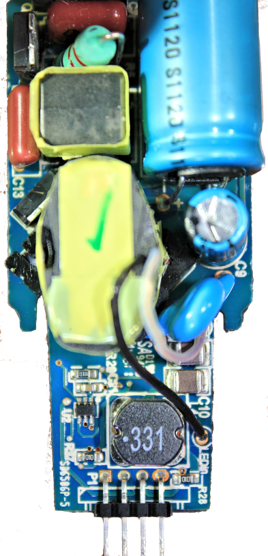
\includegraphics[height=5cm,angle=90]{./0_intro/img/LED_driver.png}};
      \begin{scope}[x={(image.south east)},y={(image.north west)}]
        \draw[red,ultra thick,rounded corners] (0.70,0.3805) rectangle (0.855,0.7);
        \draw[red,ultra thick,rounded corners] (0.11,0.1) rectangle (0.28,0.50);
        \draw[red,ultra thick,rounded corners] (0.28,0.1) rectangle (0.63,0.62);
    \end{scope}
      \end{tikzpicture}
        \caption{Magnetic components marked with a red square in a mains connected LED driver. The magnetic components dominate the volume of the converter.}
        \label{fig:smps_driver}
      \end{figure}






\section{Switched Capacitors}
Switched Capacitor Converters (SCCs) are \emph{dc-dc} power circuits composed only by switches and capacitors that provide efficient voltage conversion. SCCs have been long known and utilized, initially for voltage multiplication and more recently for voltage regulation as well. Compared to inductor based power converters, the absence of magnetic elements makes them suitable for high density power systems and integrated solutions , such as Power-System-in-Package (PSiP) or Power-System-on-Chip (PSoC).

SCCs have a fix ratio of conversion between the input and the output determined by the topology. The output voltage of the converter under no load conditions is defined as \emph{target voltage} ($v_t$), and its efficiency is very high when the load is supplied close to the \emph{target voltage}. If the output voltage goes below the \emph{target voltage} the efficiency drops, similar to the linear drivers.  The converter can not supply voltages above the \emph{target voltage}.

A common practice to extend the regulation margins of these converters is to have topologies with multiple conversion rations as shown in the plot of Fig. \ref{fig:SCC_driver}. We can see that efficiency increases as the ration $m$ gets close to the first fixed conversion ration of the converter $m_1$; right after $m_1$ the efficiency drops dramatically and it linearly increases as it approaches the second fixed conversion ratio of the converter $m_2$.

\begin{figure}[!h]
      \centering
\ctikzset { bipoles/length=1cm}
\begin{circuitikz}[scale=0.65]
\draw
    (2.5,0) to[short]
    (0,0) to[V = $V_{src}$]
    (0,3) to[short]
    (2.5,3) ;

\draw
    (2,3) --
    (2.5,3)

    (2,0) --
    (2.5,0)

    node  (IC)  at (2,0) {}
    node  (I) at (2,3) {}
    (I) to[open,v=$v_{i}$] (IC);


\draw [thick]
    (2.5,-0.5) --
    (2.5,3.5)  --
    (5.5,3.5)  --
    (5.5,-0.5) --
    (2.5,-0.5);

\draw (4,3.25)node[anchor=north]{$\frac{v_o}{v_{i}}=m$} ;

\draw (3.5,2) to[C] (3.5,0);
\draw (4.5,2) to[switch] (4.5,0);


\draw
    (5.5,0) to[short]
    (7,0) to[ leD*,v_>=$v_{o}$]
    (7,3) to[short,i_<=$i_o$]
    (5.5,3) ;


\begin{scope}[xshift = 10cm, yshift=0cm]
            \draw[->] (0,0) -- (4,0) node[anchor=north] {$  m $};
            \draw[->] (0,0) -- (0,3.2) node[anchor=east] {$\eta $};

            %Ticks X
            \draw (1.75,2pt) -- (1.75,-5pt) node[anchor=north] {$m_1$};
            \draw (3,2pt) -- (3,-5pt) node[anchor=north] {$m_2$};
            %\draw (1.5,2pt) -- (1.5,-5pt) node[anchor=north] {$0.7$};

            %Ticks Y
            \draw (2pt,2.5) -- (-5pt,2.5) node[anchor=east] {$100\%$};
            \draw (2pt,1.5) -- (-5pt,1.5) node[anchor=east] {$90\%$};

            %Markers
            \draw[dotted] (1.75,2.4) -- (1.75,0);
            \draw[dotted] (3,2.3) -- (3,0);
            \draw[dotted] (3,2.5) -- (0,2.5);
            %\draw[dotted] (1.5,1.5) -- (1.5,0);
            %\draw[dotted] (1.5,1.5) -- (0,1.5);


            \draw[thick] (0.5,1.4) -- (1.75,2.4) -- (1.75,1.6) -- (3,2.3)  node[anchor=south] {};
            %\draw[thick,dashed] (0.5,1.20) parabola[bend at end] (3,1.7)[anchor=north] {};
        \end{scope}
  \end{circuitikz}
\label{fig:inductive_smps}
\caption{Generic two port block diagram of an inductor based SMPS, and the regulation-efficacy characteristic comparing the \emph{Theoretical} limit and the \emph{Real} case. }
\end{figure}

The main advantages of these converters is that they use no inductors, which make them very favorable for integration. Integrated capacitors have a better energy density than integrated inductors. The mechanical structure of the capacitors, a stack of isolator-metal-isolator, is much easier to replicate in small scale.
Other advantage of the switch capacitors is that they divide the absolute voltage applied to the converter with the different elements, thus reducing the voltage stress in the switches and capacitors. This voltage reduction in the components is also very relevant from the point of view of integration. First, at lower voltage capacitors have better performances: more energy density, less derating and better chances of integration. Second, lower voltage switches perform better at high frequencies. And third, the lower the blocking voltage of switches is the less silicon area needed and the more standard the fabrication process is, thus reducing the production costs.

The big disadvantage of these converters is that they can not provide voltage-to-current conversion. Nevertheless, they are used for as LED driver in backlighting applications for battery supplied portable devices. In such cases, the SCCs steps-up or steps-down the battery voltage and afterwards a linear driver   provides the tight regulation that LEDs require. Adopting that architecture for general lighting could be a solution, but when we scale voltages and currents to the values used in such applications,  the number of necessary conversion steps of the SCC would make it totally infeasible and inefficient.

On the one hand, the limitation in voltage-to-current conversion would place switched capacitors out of the target architectures as power LED drivers circuits. But on the other hand, their advantageous characteristics for integration made this circuits very attractive as a possible solution for an PSoC/PSiP LED driver. Both arguments have been the motivation and the driver of the research presented in this book.

The book is divided in the four main sections that where necessary to build a switched capacitor LED driver. The first section introduces the new LED driver architecture used during the entire thesis, the \emph{Hybrid-Switched Capacitor Converter}, H-SCC from now on. The second part of this book, the core of this dissertation, presents the methodology to model H-SCC. The methodology extends the previous works in the topic providing an enhanced modeling for the design of SCCs and H-SCCs. The third section is devoted to the practical use of the new methodology, thus for the design phase of a converter. The modeling is used  to help in the development facilitating the sizing and optimization of the design variables. The last section presents a discrete implementation of 12W H-SCC LED driver and the design procedure. Although is not a regular practice, experimental work is not only presented in the in the last section. The experimental work has been used to also validate the new modeling methodology. The final section is the conclusion of the entire work and the new opportunities that can follow from it.


